\documentclass[a4paper]{article}
\usepackage[utf8]{inputenc}
\usepackage[spanish, es-tabla, es-noshorthands]{babel}
\usepackage[table,xcdraw]{xcolor}
\usepackage[a4paper, footnotesep = 1cm, width=20cm, top=2.5cm, height=25cm, textwidth=18cm, textheight=25cm]{geometry}
%\geometry{showframe}

\usepackage{tikz}
\usepackage{amsmath}
\usepackage{amsfonts}
\usepackage{amssymb}
\usepackage{float}
\usepackage{graphicx}
\usepackage{caption}
\usepackage{subcaption}
\usepackage{multicol}
\usepackage{multirow}
\setlength{\doublerulesep}{\arrayrulewidth}
\usepackage{booktabs}

\usepackage{hyperref}
\hypersetup{
    colorlinks=true,
    linkcolor=blue,
    filecolor=magenta,      
    urlcolor=blue,
    citecolor=blue,    
}

\newcommand{\quotes}[1]{``#1''}
\usepackage{array}
\newcolumntype{C}[1]{>{\centering\let\newline\\\arraybackslash\hspace{0pt}}m{#1}}
\usepackage[american]{circuitikz}
\usetikzlibrary{calc}
\usepackage{fancyhdr}
\usepackage{units} 

\graphicspath{{../Ejercicio-1/}{../Ejercicio-2/}{../Ejercicio-3/}{../Ejercicio-4/}}

\pagestyle{fancy}
\fancyhf{}
\lhead{22.01 Teoría de Circuitos}
\rhead{Mechoulam, Lambertucci, Rodriguez Turco, Londero, Galdeman}
\rfoot{\centering \thepage}
\newcommand\underrel[2]{\mathrel{\mathop{#2}\limits_{#1}}}
\begin{document}


\section{Comportamiento de Amiplificadores Operacionales.}

\subsection{Introducción}
En el presente punto se analizarán las limitaciones del amplificador operacional  \textbf{LM324} en las configuraciones inversora y no inversora.

Un amplificador operacional es un dispositivo electronico el cual dependiendo de la tension de entrada fija una tensión de salida.
El cual se puede modelar de la siguiente forma:
\begin{figure}[H]	
	\centering
	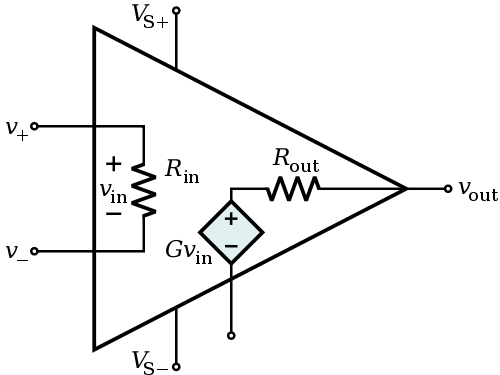
\includegraphics[width=0.7\textwidth]{Ejercicio1/Imagenes/Basicopamp.png}
	\caption{Modelo básico del amplificador operacional.}
	\label{fig:Basicopamp}
\end{figure}
donde típicamente $R_{in}\approx \infty$ y $R_{Out} \approx 0$
%%%%%%%%%%%%%%
\subsubsection{Modelo Ideal}
En el modelo ideal realimentado las hipotesis con las que se trabaja es que:
\begin{align}
V^+ = V^-\end{align}

\begin{align}V_{Out} \underrel{A_{Vol}\to \infty}{=} A_{Vol} \cdot (V^+ - V^-)\end{align}

\begin{align} R_{in}=\infty   \thinspace;\thinspace R_{Out} = 0 \end{align}
%\begin{align}  \end{align}
\subsubsection{Modelo $A_{Vol}$ finito}
Para este modelo se le agregan idealidades al modelo anterior.
\begin{align}V_{Out} = A_{Vol} \cdot (V^+ - V^-)
\label{eq:vout}
\end{align}
Si bien la realimentacion negativa intentará hacer que la diferencia entre $V^+ y V^-$ sea 0 no es algo que se va a asumir en este modelo.
\subsubsection{Modelo Polo dominante}
Este modelo es el mas cercano a la realidad que trataremos, los amplificadores operacionales poseen un polo dominante, el cual está diseñado adrede para cubrir algunos problemas que surgen
al trabajar con mayores frecuencias. Los amplificadores operacionales tienen una serie de polos debido a capacidades paracitas propias de la construccion, el  polo dominante es introducido para evitar que estos polos des-estabilicen el circuito al introducir una inversión en el lazo de realimentación 
\begin{figure}[H]	
	\centering
	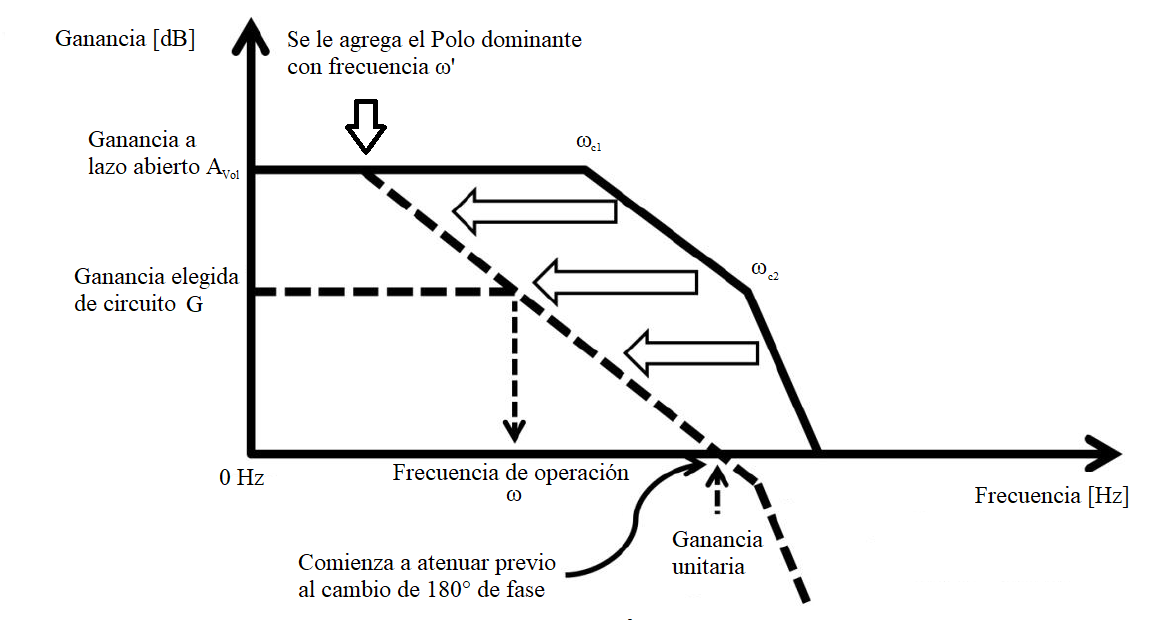
\includegraphics[width=\textwidth]{Ejercicio1/Imagenes/dompole.png}
	\caption{Modelo polo dominante.}
	\label{fig:dompole}
\end{figure}
El polo dominante soluciona estos problemas de establidad.Tambien define un Ancho de banda con el cual se puede trabajar; comunmente el dato con el que se trabaja es el GBP (Gain Bandwidth Product) el cual sigue la siguiente relación:
\begin{align} GBP= A_{Vol} \cdot \omega' \end{align}
Donde $\omega'$ es la frecuencia del polo dominante a lazo abierto.
Tambien se cumple que 
\begin{align} GBP=\omega \cdot G \end{align}
Donde $\omega$ es la frecuencia de corte del circuito en el que este aplicado y G la ganancia del mismo.
Finalmente la ecuación principal que rige este modelo es la ecuación (\ref{eq:vout}) con la singularidad de que:
\begin{align} A_{Vol} = A_{Vol}(\omega ) = \frac{A_{vol}}{1+\frac{s}{\omega '}} \end{align}

\subsection{Configuración inversora.}
El circuito propuesto por la catedra el cual será trabajado es el siguiente:

\begin{figure}[htb]	
	\centering
	\includegraphics[width=0.7\textwidth]{Ejercicio1/Imagenes/Circuitoinversor.PNG}
	\caption{Configuración inversora.}
	\label{fig:ConfInv}
\end{figure}
Para este punto se obtuvieron los siguientes datos de la hoja de datos del opamp:
\begin{table}[H]
\begin{center}
\label{tab:datos}
\begin{tabular}{|c|c|c|c|c|}
\hline
\multicolumn{5}{|c|}{\textbf{Datos}}                                      \\ \hline
\textbf{$A_{vol}$} & Max$V_{in}$ & $V_{cm}$ & Slew rate             & GBW \\ \hline
100 k              & 32V         & VCC-1.5  & 0.3 $\frac{V}{\mu s}$ & 1M  \\ \hline
\end{tabular}
\end{center}
\end{table}

%%%%%%%%%%%%%%%%%%%%%%%%%%%%
\subsubsection{Calculo Analítico del Circuito.}
Lo primero que se hizo fue utilizar el equivalente de thevenin.\\

\begin{figure}[htb]	
	\centering
	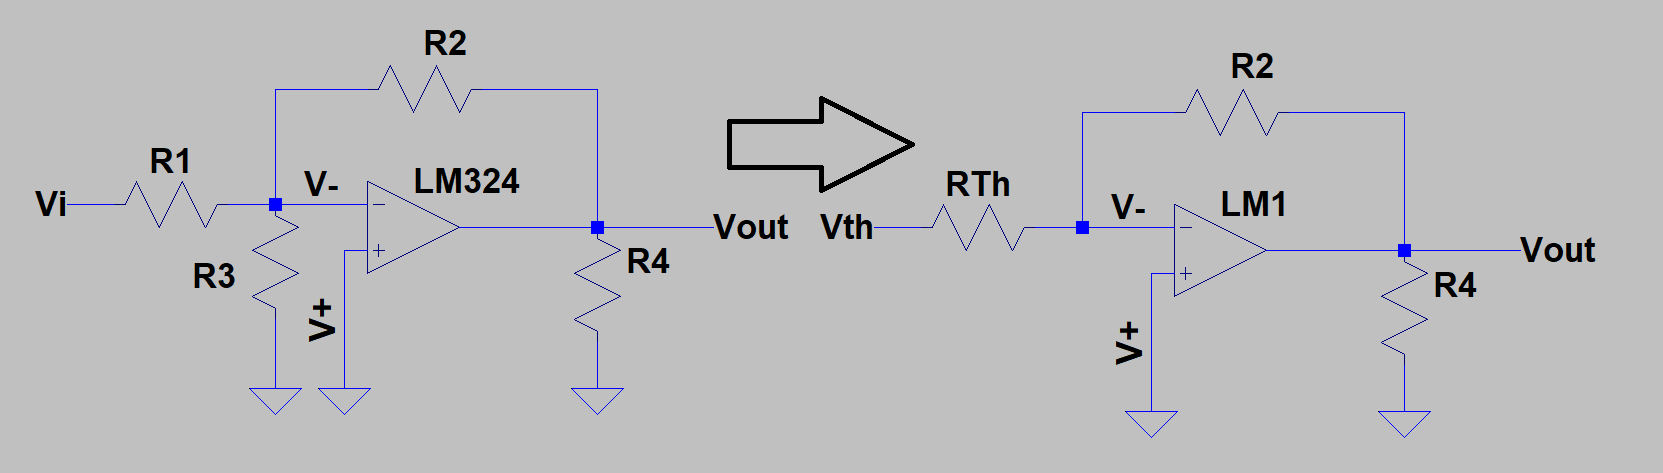
\includegraphics[width=0.7\textwidth]{Ejercicio1/Imagenes/Thevenin.PNG}
	\caption{Aplicacion teorema de Thevenin.}
	\label{fig:Thevenin}
\end{figure}

Luego de esta transformación es mas sencillo realizar los calculos analíticos.
Teniendo en cuenta que 
\begin{align}V_{Thevenin} = V_{in} \cdot \frac{R_3}{R_1+R_3}  \thinspace  R_{Thevenin} = \frac{R_1\cdot R_3}{R_1+R_3}
\label{eq:thev}
\end{align} 

El cálculo se realizara para el caso generico y una ves terminado el desarrollo se tomaran las aproximaciones para los diversos escenarios pedidos.
\begin{align}
V_{Out}= A_{Vol}(\omega) \cdot (V^+ - V^-)
\end{align}
\begin{align}
V^+=0\end{align}
\begin{align}\frac{V_{Th}-V^-}{R_{Th}}=\frac{V^--V_{Out}}{R_2}
\label{eq:nodeInv}
\end{align}
Despejando para $V_{Out}$ se llega a que:
\begin{align}
\label{eq:Vout}
V_{Out}=-V_{in} \cdot \frac{R_3}{R_1+R_3} \cdot \frac{\frac{R_2}{R_{Th}+R_2}\cdot A(\omega)}{1+\frac{R_{Th}}{R_{Th}+R_2}\cdot A(\omega)}
\end{align}
Teniendo en cuenta que la transferencia será $ H(s)=\frac{V_{Out}}{V_{in}}$.\\
Para el caso de $A_{Vol}=\infty$ simplemente bastará con tomar:
\begin{align}\lim_{A_{Vol}\to\infty} - \cdot \frac{R_3}{R_1+R_3} \cdot \frac{\frac{R_2}{R_{Th}+R_2}\cdot A(\omega)}{1+\frac{R_{Th}}{R_{Th}+R_2}\cdot A(\omega)} = -\frac{R_3}{R_1+R_3}\cdot\frac{R_2}{R_{Th}}=-\frac{R_2}{R_1}\end{align}

Para el caso de $A_{Vol}$ finito solamente se reescribira la ecuación \ref{eq:Vout}.

\begin{align}
H(s)= -\frac{R_2\cdot A_{Vol}}{R_1\cdot R_3+R_1\cdot R_3 \cdot A_{Vol} +R_2\cdot R_3+R_2\cdot R_1}
\label{eq:AvolFinite}
\end{align}

Finalmente el caso el cual incluye el polo dominante bastará con tomar 

\begin{align}A_{Vol}(\omega)=A_0 \cdot \frac{1}{1+\frac{s}{\omega'}}
\label{eq:PoloDom}
\end{align}
Donde $\omega'$ es la frecuencia del polo dominante.\\
Utilizando las ecuaciones (\ref{eq:AvolFinite}) y (\ref{eq:PoloDom})
Se llega a la expresión:
\begin{align}
\label{eq:polodom}
H(s)=-\frac{A_0R_2R_3}{A_0R_1R_3+R_1R_2+R_1R_3+R_2R_3} \cdot\frac{1}{1+\frac{s}{\omega' \cdot \frac{A_0R_1R_3+R_1R_2+R_1R_3+R_2R_3}{R_1R_2+R_1R_3+R_2R_3}}}
\end{align}

De la ecuación \ref{eq:polodom} se obtiene la frecuencia de corte del sistema.
\begin{align}
f_c=\frac{\omega'}{2\pi} \cdot \frac{A_0R_1R_3+R_1R_2+R_1R_3+R_2R_3}{R_1R_2+R_1R_3+R_2R_3}
\end{align}
Teniendo en cuenta que
\begin{align}
\omega'=\frac{GBW}{A_0} = 2 \pi\cdot 10Hz \approx 
\end{align}

Para nuestro grupo los valores de resistencias fueron los del siguiente cuadro:
\begin{table}[H]
\begin{center}
\begin{tabular}{|c|c|c|c|}
\hline
\textbf{Caso:}              & \textbf{1}               & \textbf{2}               & \textbf{3}                \\ \hline
$R_1=R_3$                   & 7k5                      & 7k5                      & 75k                       \\ \hline
$R_2$                       & 75k                      & 7k5                      & 7k5                       \\ \hline
\multicolumn{1}{|c|}{$R_4$} & \multicolumn{1}{l|}{30k} & \multicolumn{1}{l|}{30k} & \multicolumn{1}{l|}{300k} \\ \hline
\end{tabular}
\end{center}
\end{table}
Para lo cual se calculó la ganancia para el caso de $A_{Vol}$ finito e infinito y la frecuencia de corte del sistema para el caso de $A(\omega)$
\begin{table}[H]
\begin{center}
\begin{tabular}{|c|c|c|c|}
\hline
\textbf{Caso}            & \textbf{1} & \textbf{2} & \textbf{3} \\ \hline
\textbf{$H(s)_{\infty}$} & 10         & 1          & 0.1        \\ \hline
\textbf{$H(s)_{Finito}$} & 9.9998     & 0.9999     & 0.0999     \\ \hline
\textbf{$f_c$}           & 47.62KHz   & 333.34KHz  & 833.34     \\ \hline
\end{tabular}
\end{center}
\end{table}
Luego se procedió a realizar los graficos de $A_{Vol(\omega)}$ para cada uno de los 3 casos.
\begin{figure}[H]	
	\centering
	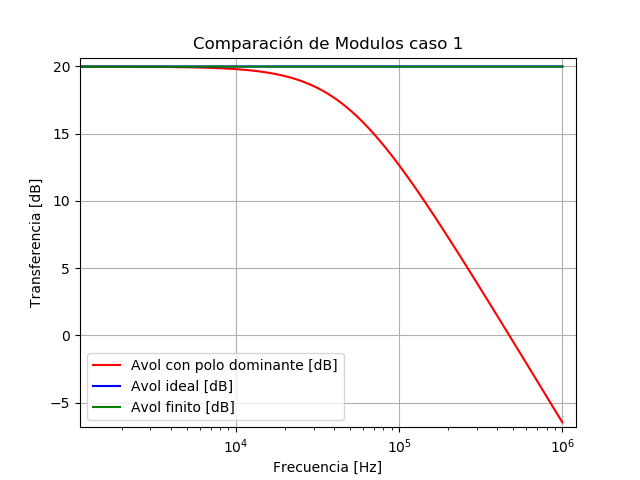
\includegraphics[width=\textwidth]{Ejercicio1/Imagenes/HCompC1.png}
	\caption{$A_{Vol(\omega)}$ Caso 1.}
	\label{fig:AvolC1}
\end{figure}
\begin{figure}[H]	
	\centering
	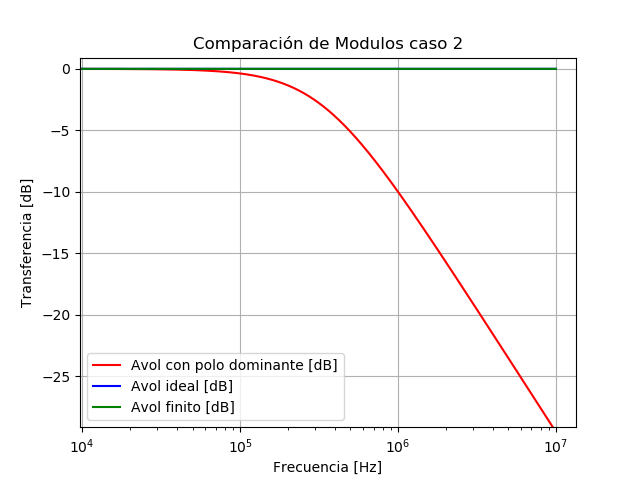
\includegraphics[width=\textwidth]{Ejercicio1/Imagenes/HCompC2.png}
	\caption{$A_{Vol(\omega)}$ Caso 2.}
	\label{fig:AvolC2}
\end{figure}
\begin{figure}[H]	
	\centering
	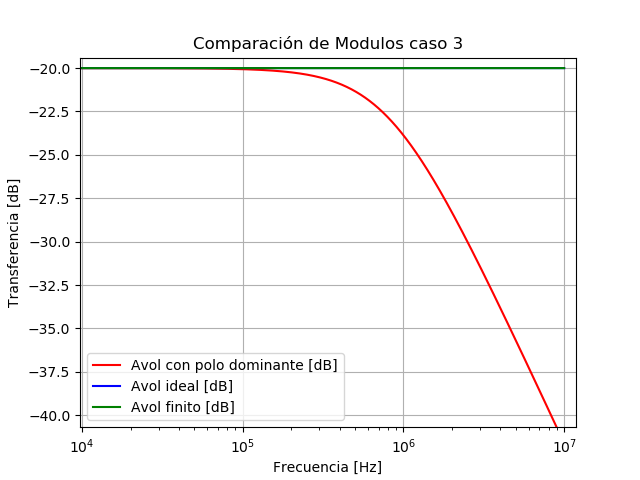
\includegraphics[width=\textwidth]{Ejercicio1/Imagenes/HCompC3.png}
	\caption{$A_{Vol(\omega)}$ Caso 3.}
	\label{fig:AvolC3}
\end{figure}
Se puede apreciar que cuanto mas baja la ganancia mayor será el ancho de banda y que a partir de la frecuencia de corte cada sistema el opamp comienza a atenuar.
El error de utilizar el caso de $A_{Vol}$ ideal en vez del caso con polo dominante se calculo como:
\begin{align}
	Error = \frac{|A_{Vol}(\omega)-A_{Vol-Ideal}|}{A_{Vol}(\omega)}
\end{align}
Obteniendo los siguientes gráficos.
\begin{figure}[H]	
	\centering
	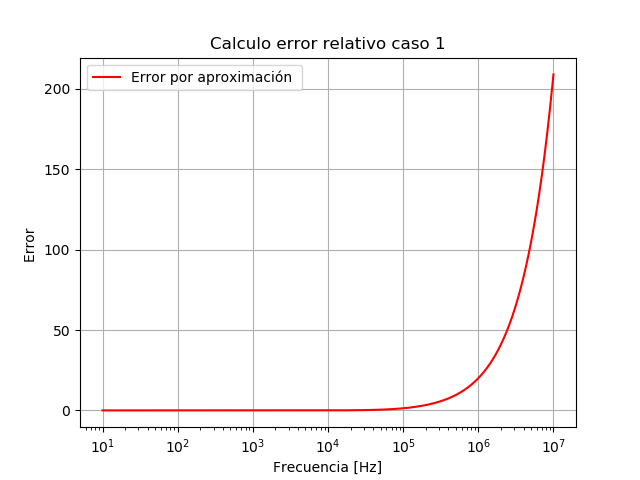
\includegraphics[width=\textwidth]{Ejercicio1/Imagenes/error1.png}
	\caption{Error relativo por aproximar Caso 1.}
	\label{fig:e1}
\end{figure}
\begin{figure}[H]	
	\centering
	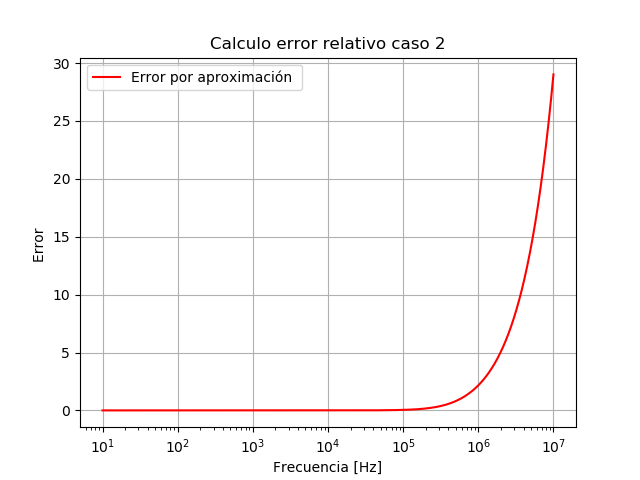
\includegraphics[width=\textwidth]{Ejercicio1/Imagenes/error2.png}
	\caption{Error relativo por aproximar Caso 2.}
	\label{fig:e2}
\end{figure}
\begin{figure}[H]	
	\centering
	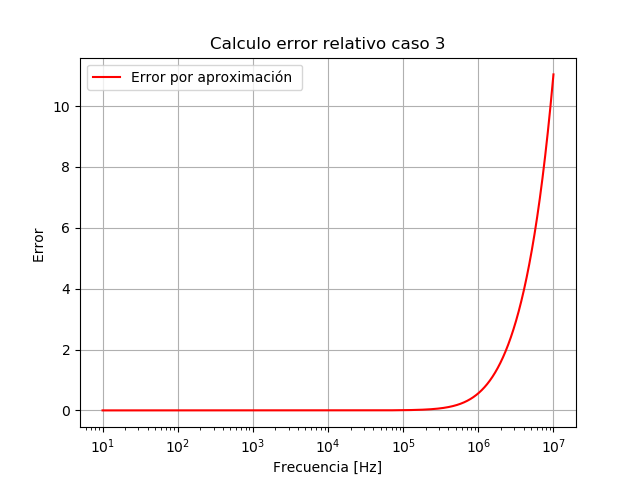
\includegraphics[width=\textwidth]{Ejercicio1/Imagenes/error3.png}
	\caption{Error relativo por aproximar Caso 3.}
	\label{fig:e3}
\end{figure}
de aqui se puede concluir que utilizar la aproximación ideal se puede utilizar siempre que se tengan en cuenta el error que uno este dispuesto a aceptar.
%%%%%%%%%%%%%%%%%%%%%%%%%%%%%%%%%%%%%%%%%%
\subsubsection{Impedancia de entrada.}

Para calcular la impedancia de entrada de los tres casos a trabajar se seguirá la misma idea de la primer parte.
\begin{align}
\label{eq:Zin}
\frac{V_{Th} - V^-}{R_{Th}}=I_{in}
\end{align}
Utilizando las ecuaciones (\ref{eq:Zin}), (\ref{eq:nodeInv}), (\ref{eq:thev}) y (\ref{eq:Vout})

Se puede llegar a la siguiente expresión:
\begin{align}
	Z_{in}(s)=\frac{A_{Vol}R_1R_3+R_1R_2+R_2R_3+R_1R_3}{A_{Vol}R_3+R_2+R_3}\cdot \frac{1+\frac{s\cdot (R_1R_2+R_1R_3+R_2R_3)}{\omega ' \cdot (A_{Vol}R_1R_3+R_1R_2+R_1R_3+R_2R_3)}}{1+\frac{s\cdot (R_2+R_3)}{\omega ' \cdot(A_{Vol}R_3+R_2+R_3)}}
\end{align}
Tambien se puede observar en la ecuación (\ref{eq:Zin}) que si $A_{Vol}$ es infinito.
\begin{align} V^- = V^+=0 \implies Z_{in}=R_1
\end{align}
Las mediciones de la impedancia de entrada se realizaron de la siguiente manera:

\begin{center}
\begin{circuitikz}[american voltages] \draw (0,0)
  node[draw,minimum width=2cm,minimum height=2.4cm] (load) {Load}
  ($(load.west)!0.75!(load.north west)$) coordinate (la)
  ($(load.west)!0.75!(load.south west)$) coordinate (lb)
  (lb) to[short,-o] ++(-0.5,0) coordinate (b) node[below] {$GND$}
  to[short] ++(-4,0) coordinate (VThb)
  to[sV=$V_{\mathrm{In}}$] (VThb |- la)
  to[R=$R$] ++(2.5,0) coordinate (VTht)
  to[short,-o,i=$I_{In}$] (VTht -| b) coordinate (a) node[above] {$A$}
  to[short] (la);
  \path (a) node[below] {$+$} -- node {$V$} (b) node[above] {$\vphantom{+}-$};
\end{circuitikz}
\end{center}
Se midio la señal de entrada y la señal en el punto A, luego se utilizó la funcion de resta del modo math del osciloscopio. Se midió el Ratio y la fase de la señal de math y la entrada. asi obteniendo un vector de medidas las cuales corresponden a la siguietne expresión.
\begin{align}
20\log\left(\frac{V_{(A-In)}}{V_{in}}\right)
\end{align}
A partir de estos valores se puede obtener la impedancia de entrada:

\begin{align}
Z_{In}=20\log\left(\frac{V_{In}}{I_{in}}\right) =20\log\left(\frac{V_{In} \cdot  R}{V_{(A-In)}}\right) = -20\log\left(\frac{V_{(A-In)}}{V_{In} }\right)+20\log (R)
\end{align}

Luego se realizaron mediciones de la impedancia de entrada y se compararon con simulaciones realizadas en \textbf{LTSpice} y el calculo analítico.
Algo a notar en los gráficos es que en el calculo analítico no fueron tomadas en cuentas las puntas del osciloscopio las cuales estaban en \textbf{x1} las cuales alteraron la medición, mientras que en las simulaciones con Spice si fueron tomadas en cuenta.
\begin{figure}[H]	
	\centering
	
\includegraphics[width=0.9\textwidth]{Ejercicio1/Imagenes/ZinC1.png}
	\caption{Impedancia de entrada Caso 1.}
	\label{fig:CompZinC1}
\end{figure} 

\begin{figure}[H]	
	\centering
	
\includegraphics[width=0.9\textwidth]{Ejercicio1/Imagenes/CZinC2.png}
	\caption{Impedancia de entrada Caso 2.}
	\label{fig:CompZinC2}
\end{figure} 
\begin{figure}[H]	
	\centering
	
\includegraphics[width=\textwidth]{Ejercicio1/Imagenes/CZinC3.png}
	\caption{Impedancia de entrada Caso 3.}
	\label{fig:CompZinC3}
\end{figure} 

\begin{figure}[H]	
	\centering
	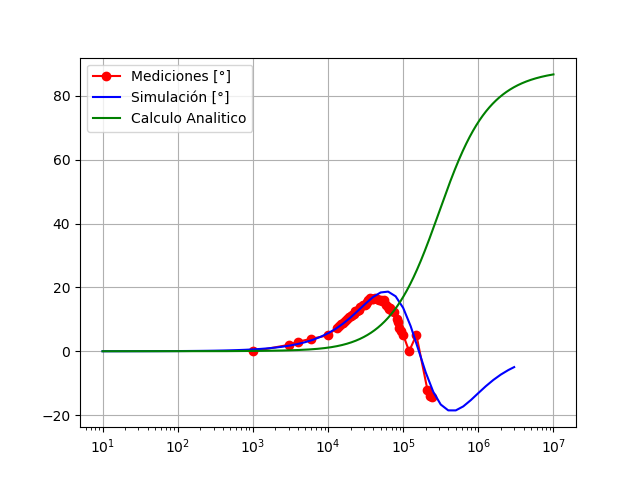
\includegraphics[width=0.9\textwidth]{Ejercicio1/Imagenes/ZinphC1.png}
	\caption{Impedancia de entrada Caso 1.}
	\label{fig:CompZinphC1}
\end{figure} 

\begin{figure}[H]	
	\centering
	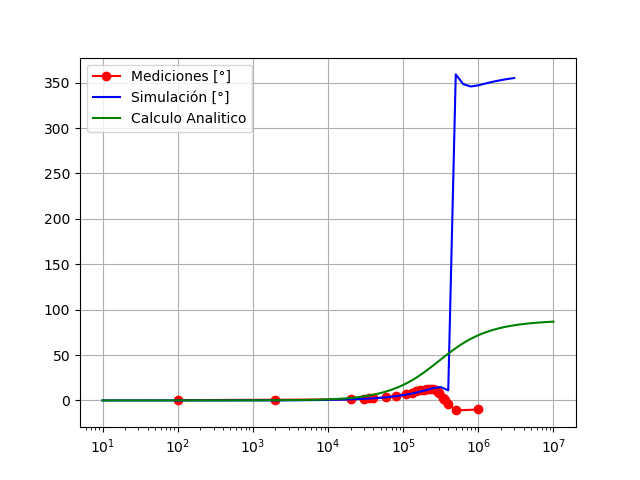
\includegraphics[width=0.9\textwidth]{Ejercicio1/Imagenes/ZinphC2.png}
	\caption{Impedancia de entrada Caso 2.}
	\label{fig:CompZinphC2}
\end{figure} 
\begin{figure}[H]	
	\centering
	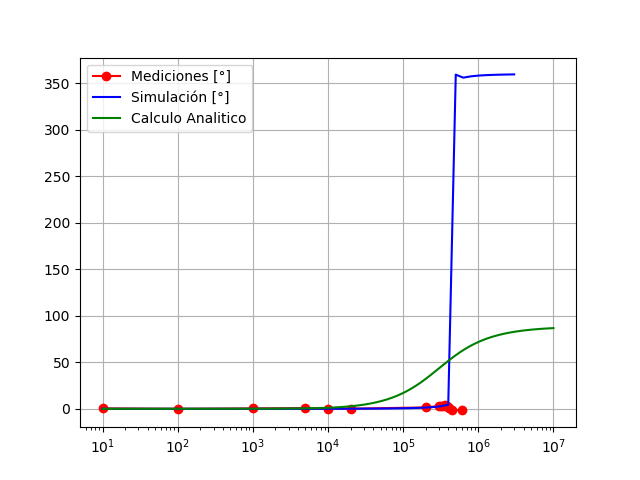
\includegraphics[width=\textwidth]{Ejercicio1/Imagenes/ZinphC3.png}
	\caption{Impedancia de entrada Caso 3.}
	\label{fig:CompZinphC3}
\end{figure} 
Tambien cabe destacar que en los graficos (\ref{fig:CompZinphC2}) y (\ref{fig:CompZinphC3}) realmente no hay un salto sino que esta desfasado 360=0
%%%%%%%%%%%%%%%%%%%%%%%%%%%%%%
\subsubsection{Máximos valores de entrada.}
El máximo valor de entrada a partir del cual el Opamp satura estará definido por diversas variables, siendo algunas de ellas la amplitud de entrada de la señal, la ganancia del sistema y la frecuencia de entrada.

Para buscar estos valores nos centraremos en los 3 casos a analizar. 
Asumiendo el opamp con ganancia ideal y sabiendo que:
\begin{align} V_{Out}=H(s)\cdot V_{in}\end{align}
El máximo valor de $V_{in}$ quedará definido por la tensión de saturación del opamp. Que para el \textbf{LM324} es VCC-1.5 lo cual para nuestro caso será 13.5V\footnote{Esta información fue extraida de la hoja de datos}
Luego utilizando esta relación se realizó el siguiente cuadro para las distintas ganancias que utilizaremos\footnote{Para el caso 3 si bien matemáticamente la máxima $V_{in}$ es 135V en la hoja de datos nos informa que el máximo que soporta el dispositivo sin quemarse es de 32V }.
\begin{table}[H]
\begin{center}
\label{tab:maxin}
\begin{tabular}{|c|c|c|c|}
\hline
\textbf{Caso:}        & \textbf{1} & \textbf{2} & \textbf{3} \\ \hline
\textbf{Ganancia ideal}     & 10         & 1          & 0.1        \\ \hline
\textbf{$V_{in-Max}$} & 1.35       & 13.5       & 32         \\ \hline
\end{tabular}
\end{center}
\end{table}
Luego se graficó la maxima tension de entrada en funcion de la ganancia:
\begin{figure}[H]	
	\centering
	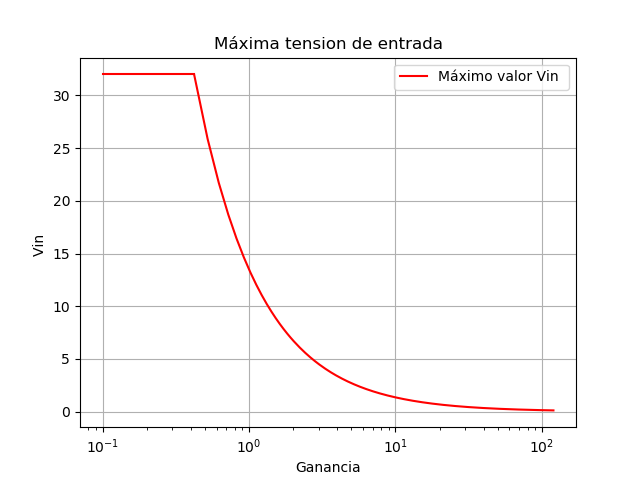
\includegraphics[width=\textwidth]{Ejercicio1/Imagenes/maxvin.png}
	\caption{Maxima tensión de entrada en funcion de la Ganancia.}
	\label{fig:MaxVin}
\end{figure} 
Tambien se analizó la máxima amplitud de entrada en funcion de la frecuencia tal que no haya slew-rate \footnote{el cual es un efecto que se detallará luego en su propia sección} ni saturación.
La cual puede ser apreciada en el siguiente gráfico:
\begin{figure}[H]	
	\centering
	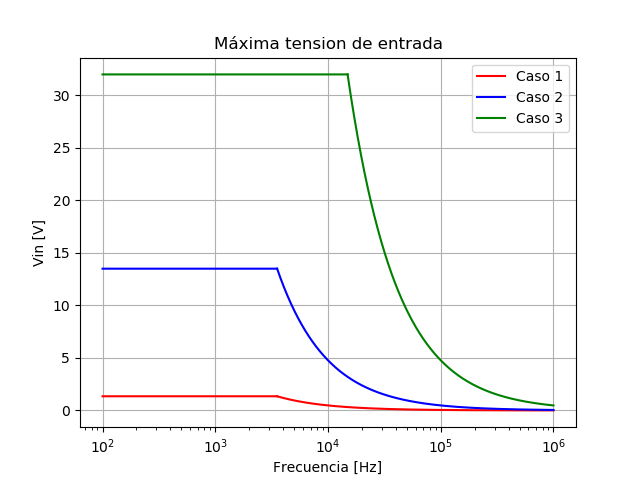
\includegraphics[width=\textwidth]{Ejercicio1/Imagenes/maxvinsr.png}
	\caption{Maxima tensión de entrada sin saturación ni slew-rate.}
	\label{fig:MaxVinsr}
\end{figure} 
%%%%%%%%%%%%%%%%%%
\subsubsection{Principales Caracteristicas.}
En el caso que $R_3$ sea igual a 0 a la salida del opamp deberia haber 0V, esto no es la realidad dado a que existe una tensión de offset la cual será analizada en la seccion 3 de este informe.
El proposito de $R_4$ a primera vista no es evidente dado que la transferencia es independiente de ella, pero observando que existe una corriente máxima\footnote{Obteniendo el valor de la datasheet se sabe que $I_{Max}=20mA$} que puede aportar el opamp se llego a  que el proposito de $R_4$ es limitar la corriente por lo tanto su valor debe ser $R_4>\frac{V_{Out}}{I_{Max}}$ 
%%%%%%%%%%%%%%%%%%%%
\subsubsection{DC-Sweep.}
Se realizó un barrido entre -VCC y VCC utilizando un generador de funciones con una rampa y un circuito inversor para llegar a la tension de salida necesitada dado a que el generador de funciones solo puede entregar 20Vpp.
El comportamiento del opamp no es lineal para todo el rango de entradas, su comportamiento lineal se puede observar unicamente en el rango entre -Vsat y Vsat, tenienod tensiones de entrada máxima para cada caso las que se observan en la figura (\ref{fig:MaxVinsr})
Se registraron las siguientes mediciones:
\begin{figure}[H]	
	\centering
	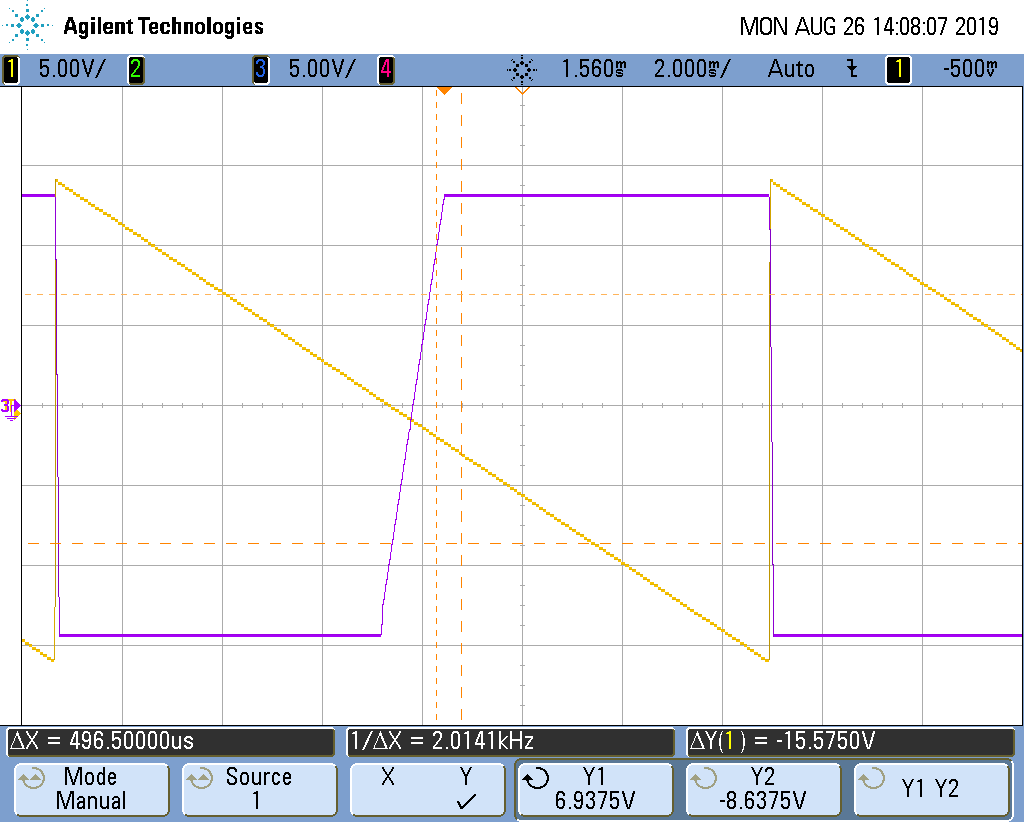
\includegraphics[width=\textwidth]{Ejercicio1/Imagenes/dc_sweep_c1.png}
	\caption{DC-sweep Caso 1.}
	\label{fig:dcc1}
\end{figure} 
Se puede observar en este caso como el opamp satura a partir de una rension mayor a 1.35 Volts como se predijo en le punto (a)
\begin{figure}[H]	
	\centering
	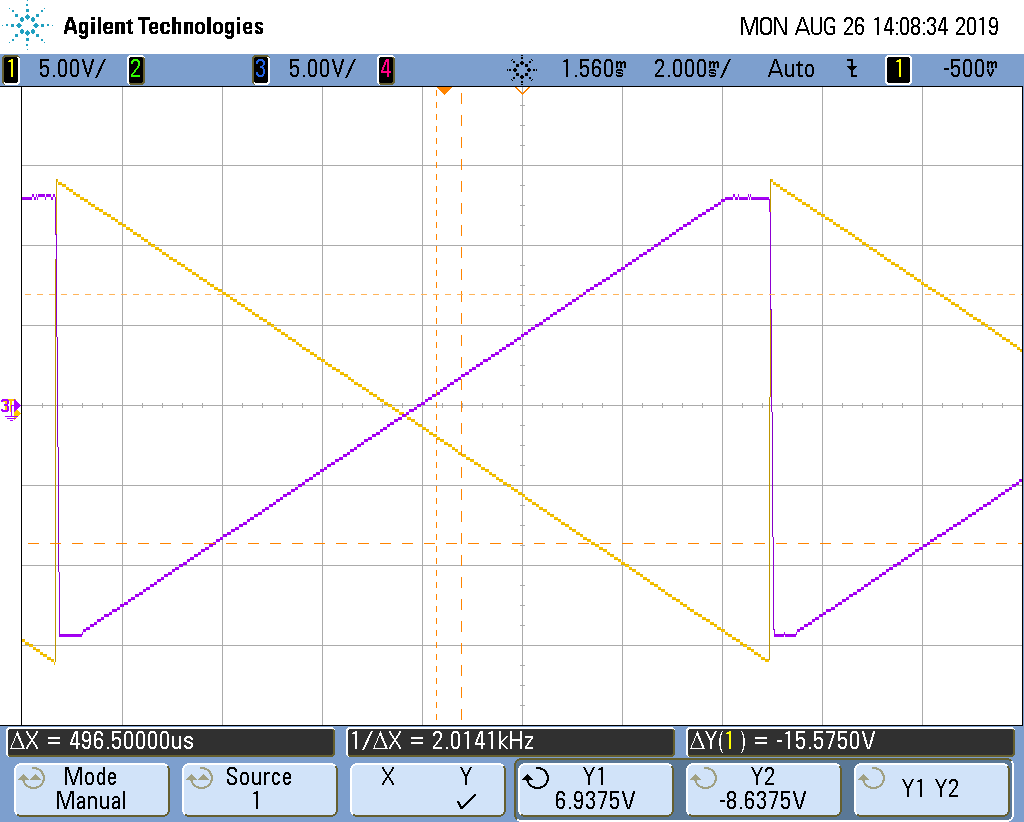
\includegraphics[width=\textwidth]{Ejercicio1/Imagenes/dc_sweep_c2.png}
	\caption{DC-sweep Caso 2.}
	\label{fig:dcc2}
\end{figure} 
En esta figura se ve como el comportamiento del opamp es lineal en la mayoria del espectro expeto en las puntas donde alli lo deja de ser como fue predicho en el punto (a) a unos $\approx$ 13.5 V
\begin{figure}[H]	
	\centering
	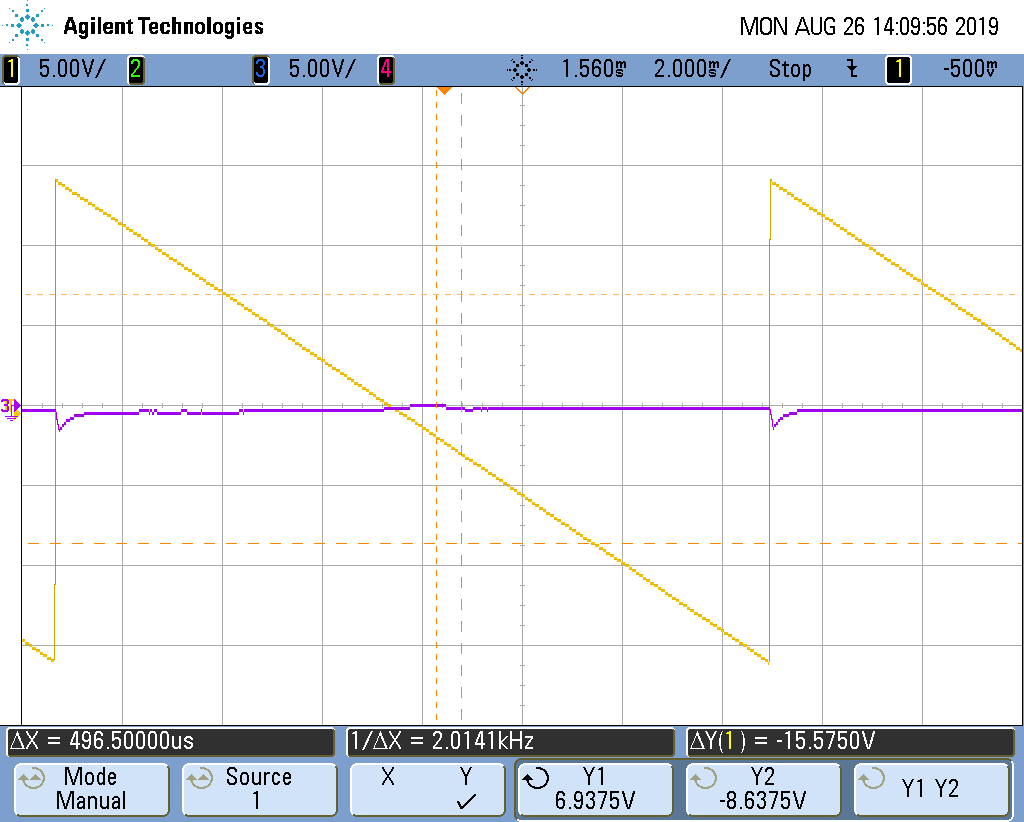
\includegraphics[width=\textwidth]{Ejercicio1/Imagenes/dc_sweep_c3.png}
	\caption{DC-sweep Caso 3.}
	\label{fig:dcc3}
\end{figure} 
Finalmente en esta figura se ve que el opamp tiene comportamiento lineal para todos los valores de la rampa
Otro efecto alineal del amplificador operacional que fue observado es el efecto de Cross-over el cual es introducido dado a la polarización de los transistores que tiene por dentro el operacional , uno puede evitar tener que lidear con ese problema al agregar una tensión de offset de continua que baste para polarizar los transistores, en este trabajo los valores utilizados fueron 0.7V ó 1.4V.
%%%%%%%%%%%%%%%%%%%%%%%%%%
\subsubsection{Slew-Rate.}
El slew-rate esta definido como la máxima variación temporal de la salida del opamp. El slew-Rate depende de 3 parametros siendo estos la frecuencia, la amplitud y la ganancia; esto siendo para una senoidal, pero dado que se puede desdcribir cualquier señal como una combinación lineal de senos se puede decir que el slewrate de una señal arbitraria tambien dependerá de estos parametros.
Si se le demanda a l opamp una tasa de cambio mayor a la soportada por le SR procedera a distorcionar la señal.
\begin{align}  SR= Max\left( \frac{\partial V_{Out}}{\partial t}\right)  \end{align}
Utilizando una entrada senoidal de la forma.
$$V_{in}=A\cdot \sin (\omega t)$$
\begin{align}   SR= Max\left( \frac{\partial (G\cdot A\cdot \sin (\omega t))}{\partial t}\right) = A \cdot \omega \cdot G  
\label{eq:sr}
\end{align}
A partir de la expresión  (\ref{eq:sr}) se llega a una relacion que debe cumplir la señal de entrada para no presentar efectos de slew-rate. Esta limitacion tiene un grado de libertad, por lo tanto se puede elegir un parametro fijo y regular el otro, por ejemplo fijando la frecuencia de entrada se debera cumplir que:
\begin{align} V_{in}	\leq \frac{SR}{G\cdot \omega_0}\end{align}
Se midió el Slew-Rate  utilizando como entrada una senoidal obteniendo la siguiente medición:
\begin{figure}[H]	
	\centering
	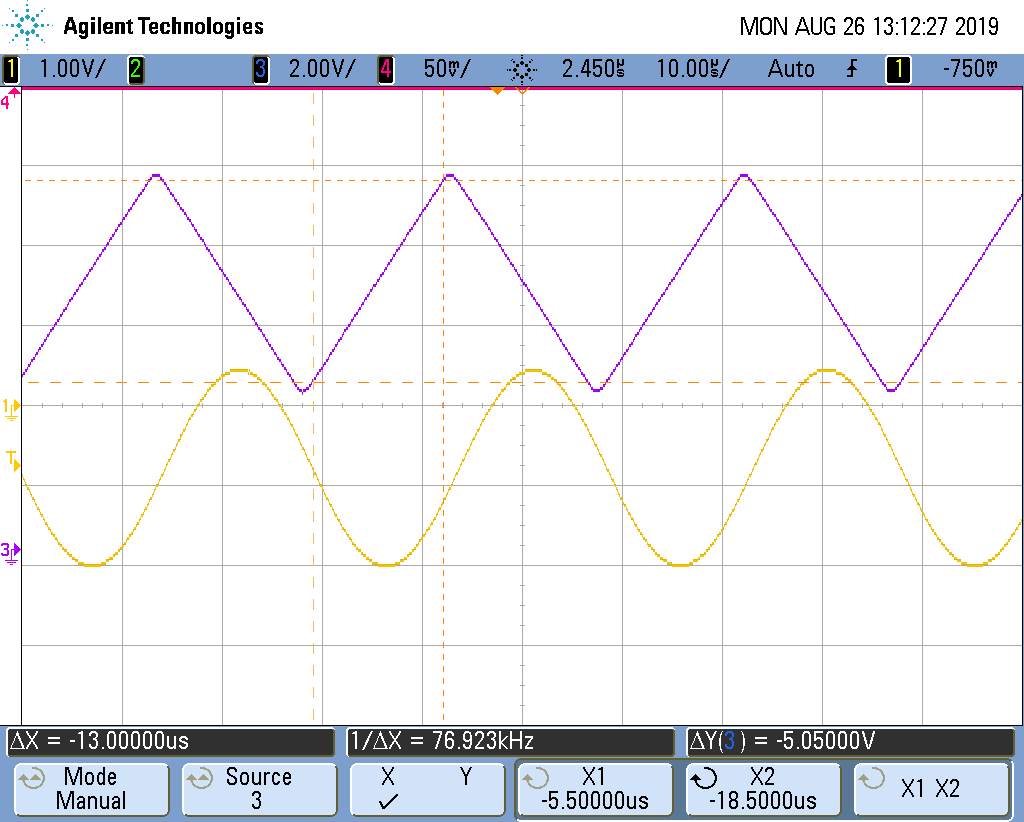
\includegraphics[width=\textwidth]{Ejercicio1/Imagenes/slew_rate1.png}
	\caption{Medición Slew-Rate.}
	\label{fig:SlewRate}
\end{figure}
De aqui utilizando la ecuación (\ref{eq:sr}) se obtiene que:
\begin{align}
SR \approx  0.38 \frac{V}{\mu s}
\end{align}
lo cual concuerda con lo provisto por el fabricante de la tabla (\ref{tab:datos})
%%%%%%%%%%%%%%%%%%%%%%%%%%%%%%%%%%%%
\subsubsection{Respuesta en frecuencia.}
Se midió la respuesta en frecuencia de la configuración en los diversos casos y se grafico junto a simulaciones hechas en spice y el calculo teórico.
\begin{figure}[H]	
	\centering
	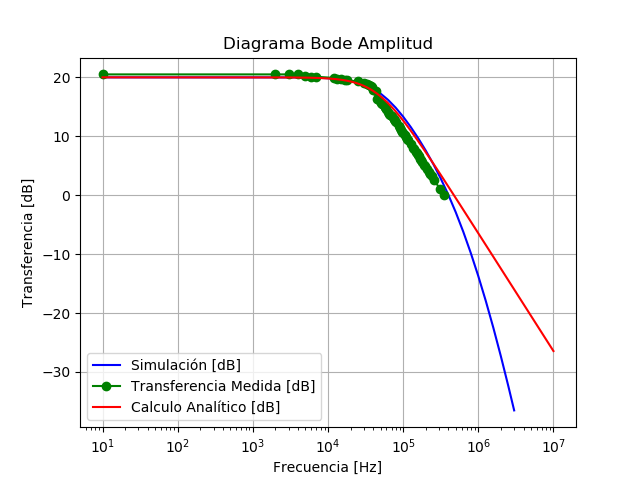
\includegraphics[width=\textwidth]{Ejercicio1/Imagenes/BodeC1.png}
	\caption{Diagrama de Bode Amplitud Caso 1.}
	\label{fig:BodeC1}
\end{figure} 
\begin{figure}[H]	
	\centering
	
\includegraphics[width=\textwidth]{Ejercicio1/Imagenes/BodephC1.png}
	\caption{Diagrama de Bode fase Caso 1.}
	\label{fig:BodephC1}
\end{figure} 
En estas mediciones el principal problema que se presento fue el hecho de que habia que lidear con que el opamp saturaba, se hacian evidentes los efectos del slew-rate  dado a que esta configuracion amplifica y efecto de  Cross-over. Tambien un problema fue que dada que la tensiond e entrada era tan pequeña como se puede apreciar en la figura (\ref{fig:MaxVinsr}), la señal se encontraba con ruido el cual era amplificado y se obtenia mayor ruido a la salida.
\begin{figure}[H]	
	\centering
	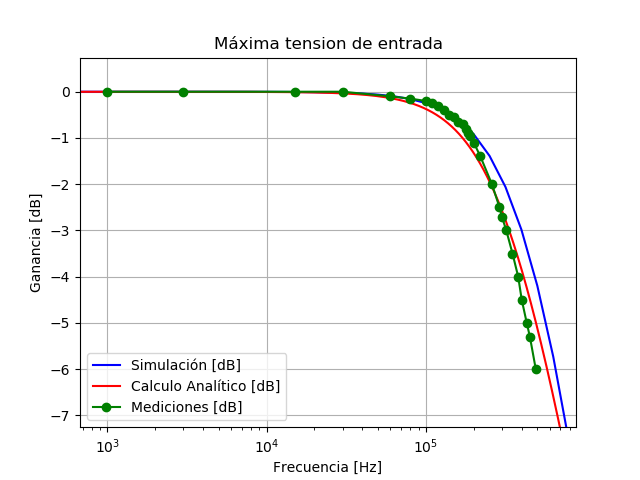
\includegraphics[width=\textwidth]{Ejercicio1/Imagenes/BodeC2.png}
	\caption{Diagrama de Bode Amplitud Caso 2.}
	\label{fig:BodeC2}
\end{figure} 
\begin{figure}[H]	
	\centering
	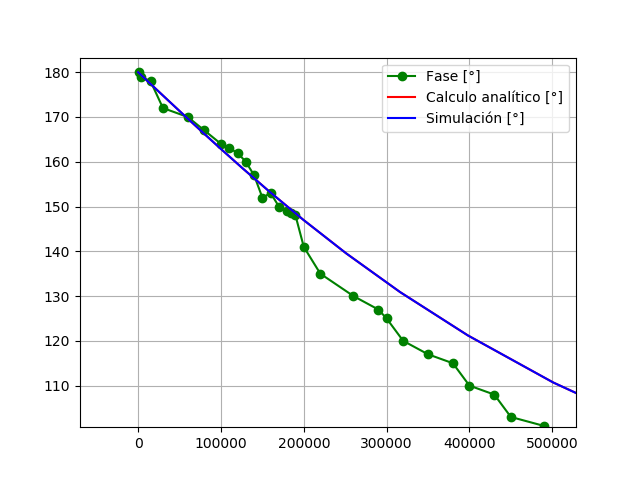
\includegraphics[width=\textwidth]{Ejercicio1/Imagenes/BodephC2.png}
	\caption{Diagrama de Bode fase Caso 2.}
	\label{fig:BodephC2}
\end{figure} 
Aqui deberia decir algo util
\begin{figure}[H]	
	\centering
	
\includegraphics[width=\textwidth]{Ejercicio1/Imagenes/BodeC3.png}
	\caption{Diagrama de Bode Amplitud Caso 3.}
	\label{fig:BodeC3}
\end{figure} 
\begin{figure}[H]	
	\centering
	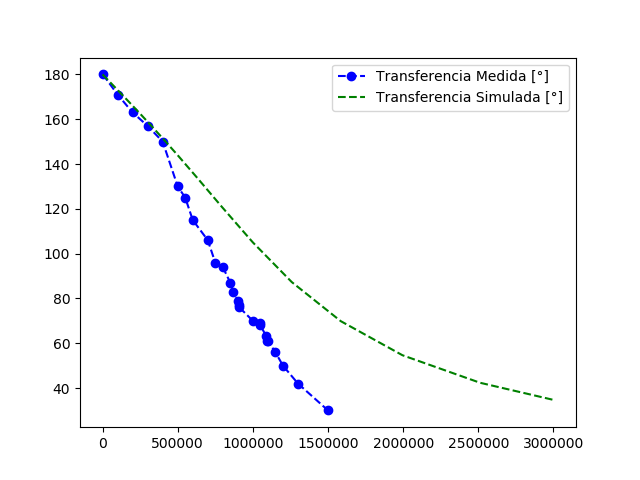
\includegraphics[width=\textwidth]{Ejercicio1/Imagenes/BodephC3.png}
	\caption{Diagrama de Bode fase Caso 3.}
	\label{fig:BodephC3}
\end{figure} 
Para las mediciones del tercer caso se presento el problema de que al estar atenuando y la señal a medir se encontraba cerca del pisod e ruido a altas frecuencias y era complicado realizar las mediciones. Algo que se puede apreciar en esta medicion es la aparición de un sobrepico ne las mediciones. Estas mediciones fueron hechas con una punta \textbf{x10} la cual introdujo un polo mas y se armó un sistema de segundo orden el cual agrega el sobrepico.
\subsubsection{Concluciones.}
\subsection{Configuración No-inversora.}
\end{document}